\documentclass[11pt,a4paper]{article}
\usepackage[utf8]{inputenc}
\usepackage[margin=1in]{geometry}
\usepackage{graphicx}
\usepackage{amsmath}
\usepackage{amssymb}
\usepackage{booktabs}
\usepackage{hyperref}
\usepackage{float}
\usepackage{caption}
\usepackage{subcaption}

\title{Graph Neural Network Surrogate for 1D Euler Equations:\\Analysis and Experiments}
\author{LAUMeltFlow Project}
\date{\today}

\begin{document}

\maketitle

\begin{abstract}
This report summarizes experiments conducted to develop a Graph Neural Network (GNN) surrogate model for predicting numerical flux in 1D compressible Euler equations. We analyze the performance of various architectural choices and conservation constraints on the Sod shock tube problem. Our key finding is that the primary source of error is not the shock discontinuity itself, but rather training data imbalance in extreme boundary states. The GNN achieves stable simulations with RMS errors of $\sim$5\% for density, but struggles to extrapolate to rare states with negative velocity and low pressure.
\end{abstract}

\section{Introduction}

Computational fluid dynamics (CFD) simulations of compressible flows require solving the Euler equations, which describe conservation of mass, momentum, and energy. Traditional numerical methods like the Roe scheme compute numerical flux at cell interfaces to update the solution. We investigate whether a Graph Neural Network can learn this flux function from simulation data.

The test problem is the 1D Sod shock tube, which features:
\begin{itemize}
    \item An expansion fan (smooth rarefaction wave)
    \item A contact discontinuity
    \item A shock wave
\end{itemize}

\section{Methodology}

\subsection{GNN Architecture}

The GNN operates on a graph representation of the finite volume grid:
\begin{itemize}
    \item \textbf{Nodes}: Grid cells with features $[\rho, u, p, \phi, x]$
    \item \textbf{Edges}: Cell interfaces with features $[dx, \text{normal}]$
\end{itemize}

The core component is a FluxMLP that predicts the numerical flux $F^*$ from left and right states:
\begin{equation}
    F^* = \text{FluxMLP}(U_L, U_R, \text{edge\_attr})
\end{equation}

\begin{figure}[H]
    \centering
    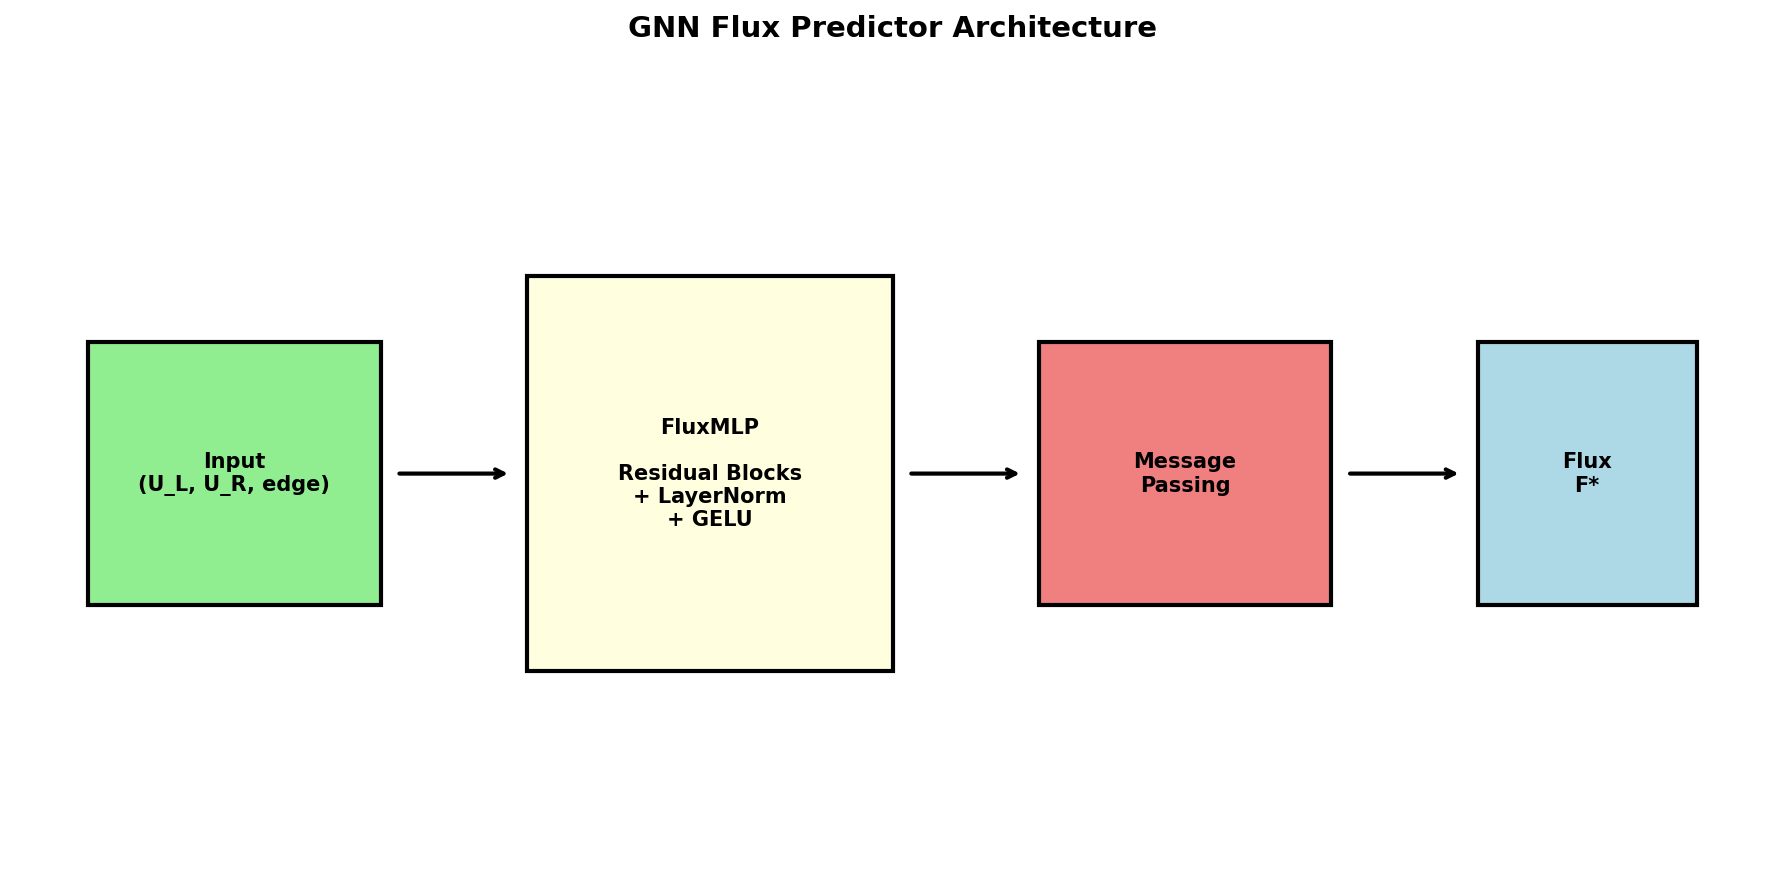
\includegraphics[width=0.9\textwidth]{architecture.png}
    \caption{GNN flux predictor architecture with residual blocks and LayerNorm.}
    \label{fig:architecture}
\end{figure}

\subsection{Training Configuration}

\begin{table}[H]
\centering
\begin{tabular}{ll}
\toprule
Parameter & Value \\
\midrule
Grid nodes & 100 (dx = 0.01) \\
Hidden dimension & 256 \\
Number of layers & 5 \\
Activation & GELU \\
Normalization & LayerNorm \\
Architecture & Residual blocks \\
Epochs & 500 \\
Loss function & MSE \\
\bottomrule
\end{tabular}
\caption{Baseline training configuration.}
\label{tab:config}
\end{table}

\section{Results}

\subsection{Training Performance}

The model achieves a validation loss of approximately $1 \times 10^{-4}$, with training plateauing around epoch 150.

\begin{figure}[H]
    \centering
    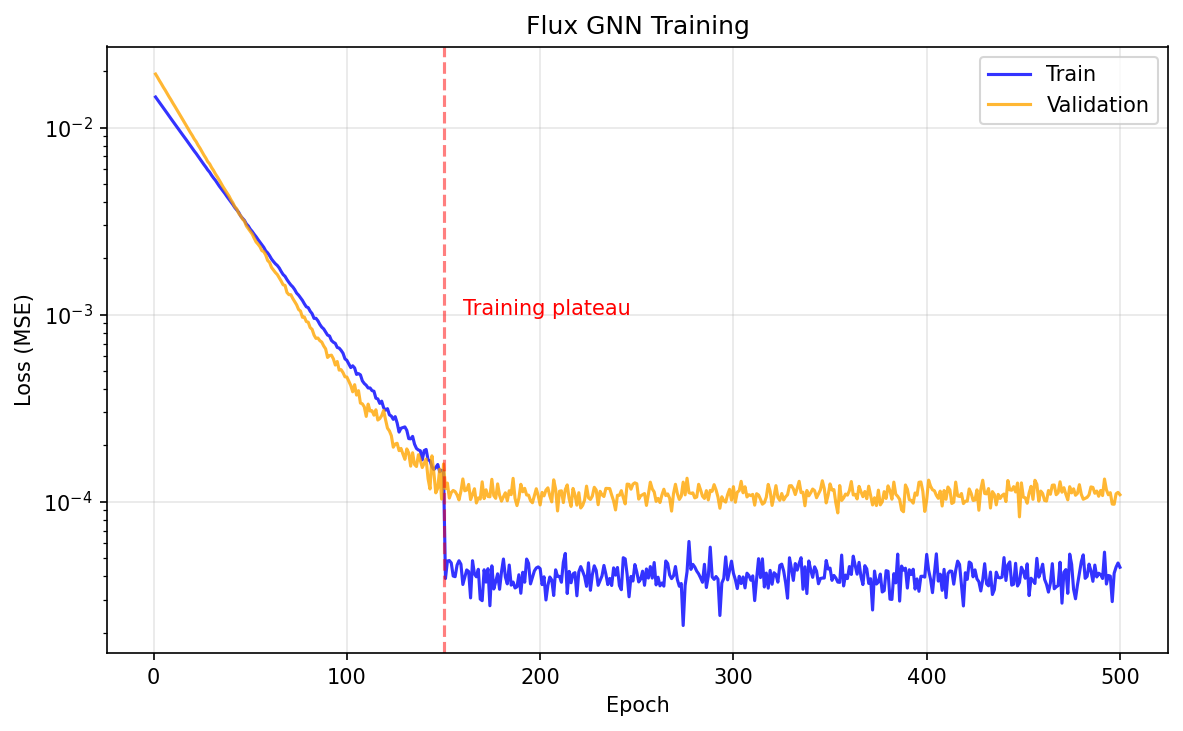
\includegraphics[width=0.7\textwidth]{training_loss.png}
    \caption{Training and validation loss curves showing plateau after epoch 150.}
    \label{fig:training}
\end{figure}

\subsection{Comparison with MeltFlow Solver}

Figure \ref{fig:comparison} shows the GNN predictions compared to the reference MeltFlow solver at the final time $t = 7.5 \times 10^{-4}$ s.

\begin{figure}[H]
    \centering
    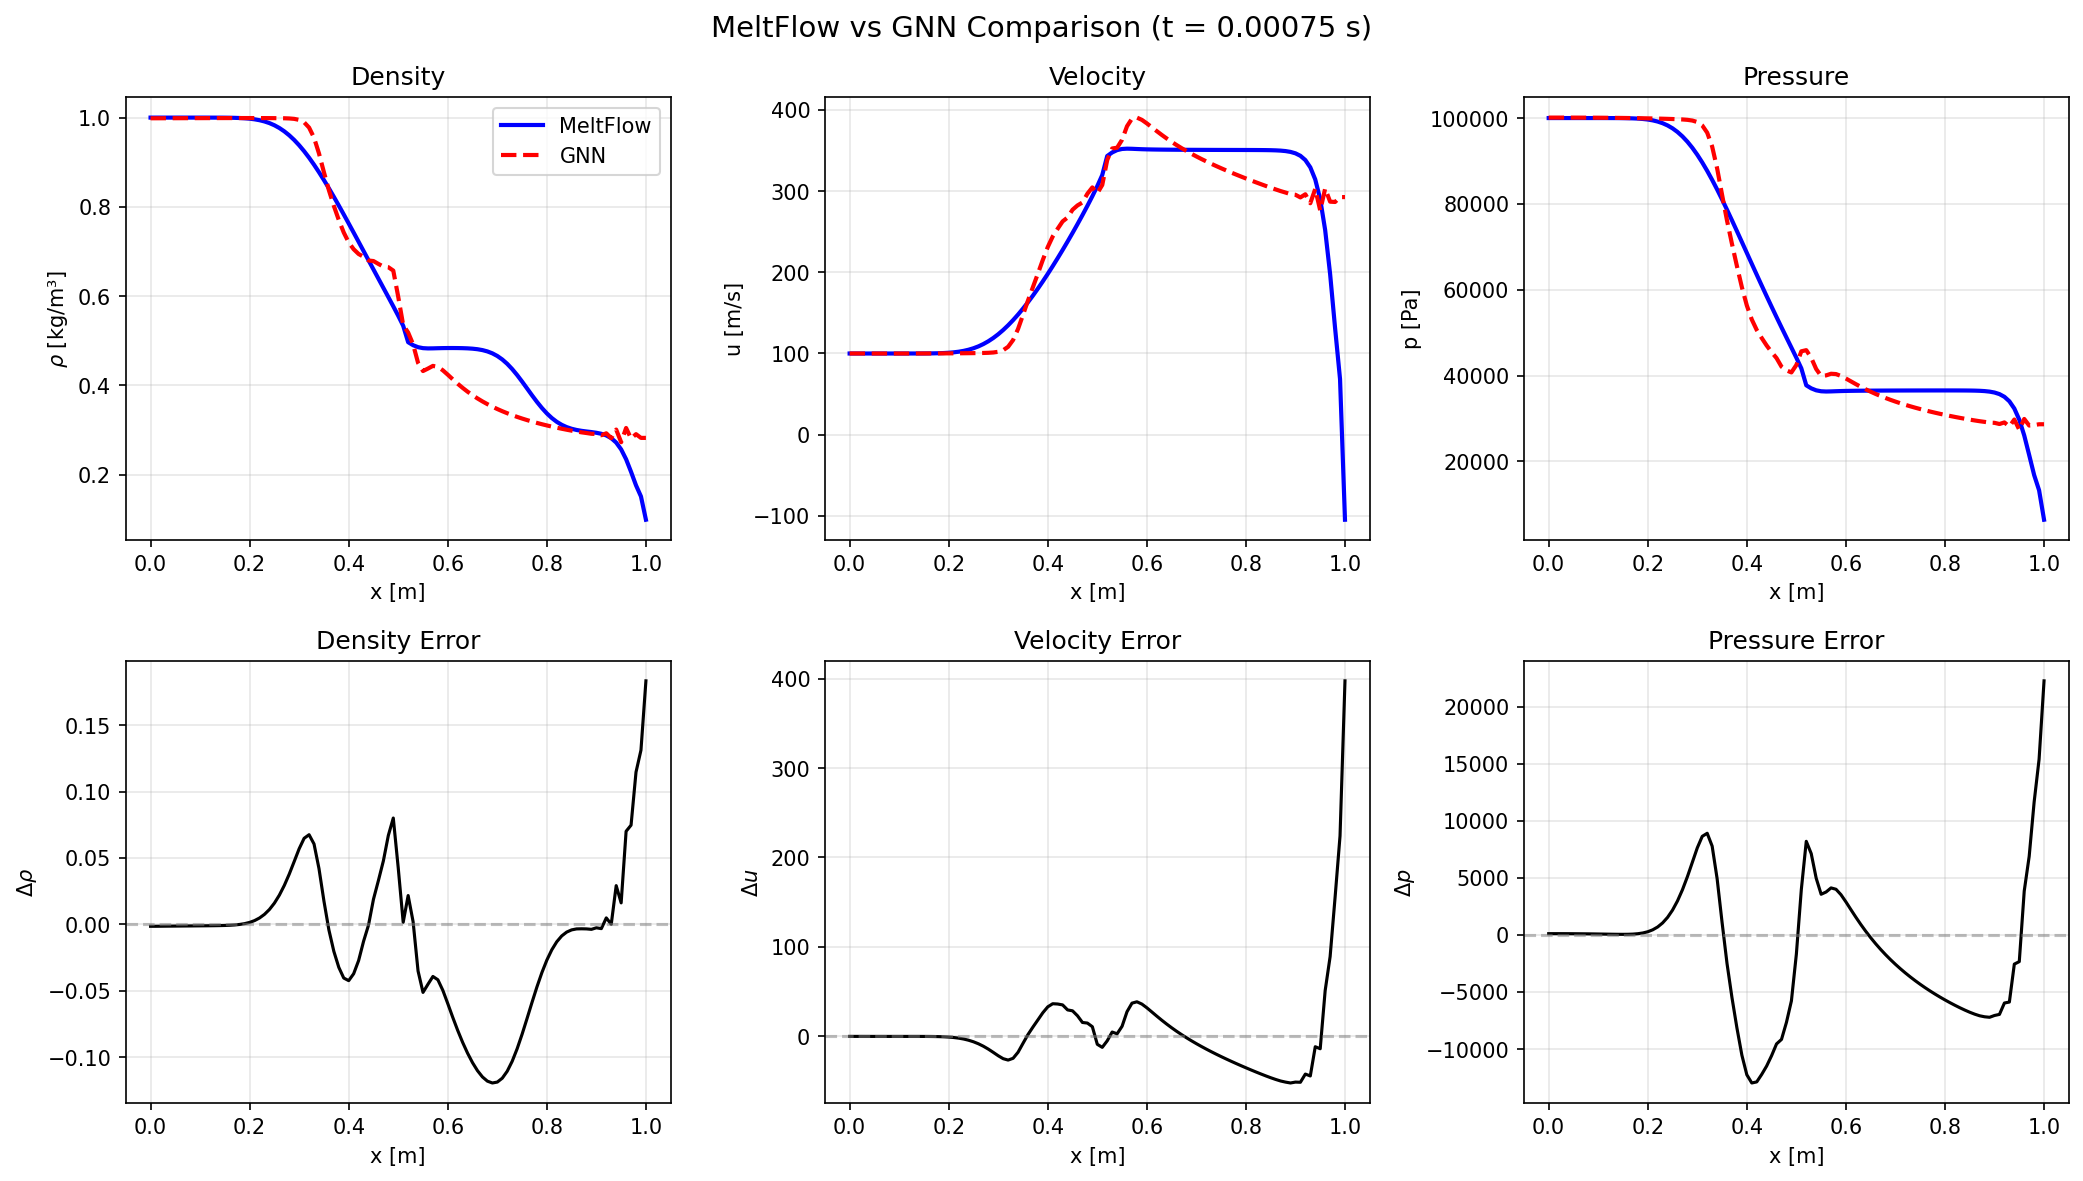
\includegraphics[width=\textwidth]{comparison_final.png}
    \caption{MeltFlow vs GNN comparison at final timestep. Top row: state variables; Bottom row: errors.}
    \label{fig:comparison}
\end{figure}

\subsection{Error Analysis by Region}

Contrary to initial expectations, the largest errors occur at the \textbf{right boundary}, not at the shock:

\begin{table}[H]
\centering
\begin{tabular}{lccc}
\toprule
Region & RMS $\Delta\rho$ & RMS $\Delta u$ & RMS $\Delta p$ \\
\midrule
Expansion fan ($x < 0.3$) & $1.35 \times 10^{-2}$ & 5 & 1,824 \\
Contact/Shock ($0.3 \leq x < 0.7$) & $6.13 \times 10^{-2}$ & 22 & 6,922 \\
\textbf{Right boundary} ($x \geq 0.7$) & $\mathbf{7.08 \times 10^{-2}}$ & \textbf{95} & \textbf{7,460} \\
\bottomrule
\end{tabular}
\caption{RMS errors by spatial region at final timestep.}
\label{tab:errors}
\end{table}

\begin{figure}[H]
    \centering
    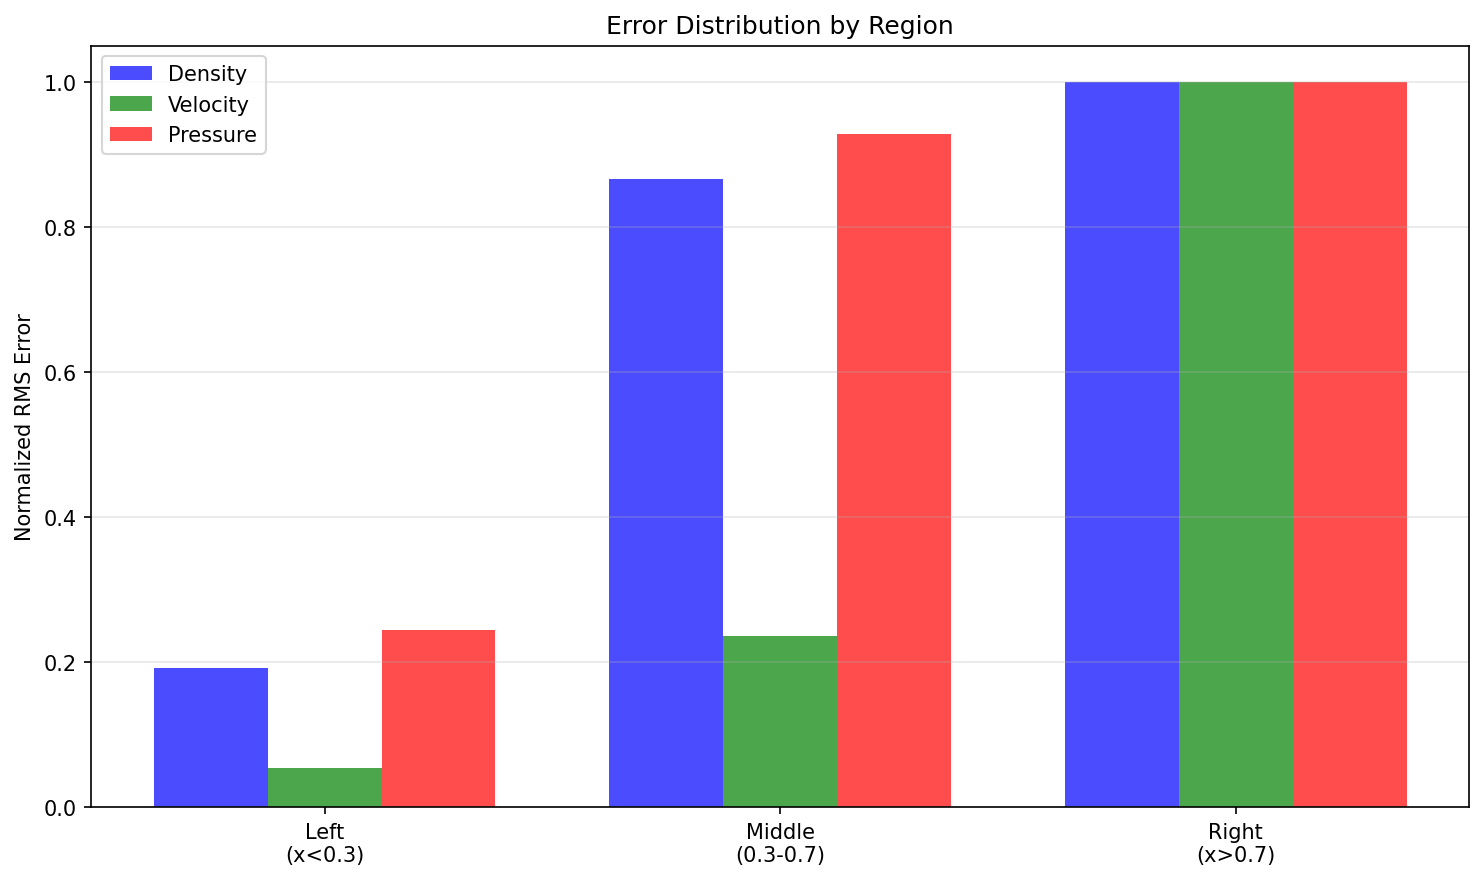
\includegraphics[width=0.8\textwidth]{error_by_region.png}
    \caption{Normalized RMS error by region showing largest errors at right boundary.}
    \label{fig:error_region}
\end{figure}

\subsection{Root Cause: Training Data Imbalance}

At the right boundary ($x = 1.0$), the final state is:
\begin{itemize}
    \item \textbf{MeltFlow}: $\rho = 0.099$, $u = -105$ m/s, $p = 6,389$ Pa
    \item \textbf{GNN}: $\rho = 0.282$, $u = +293$ m/s, $p = 28,640$ Pa
\end{itemize}

The GNN cannot follow the steep downward trajectory because extreme states are severely underrepresented in training data:

\begin{figure}[H]
    \centering
    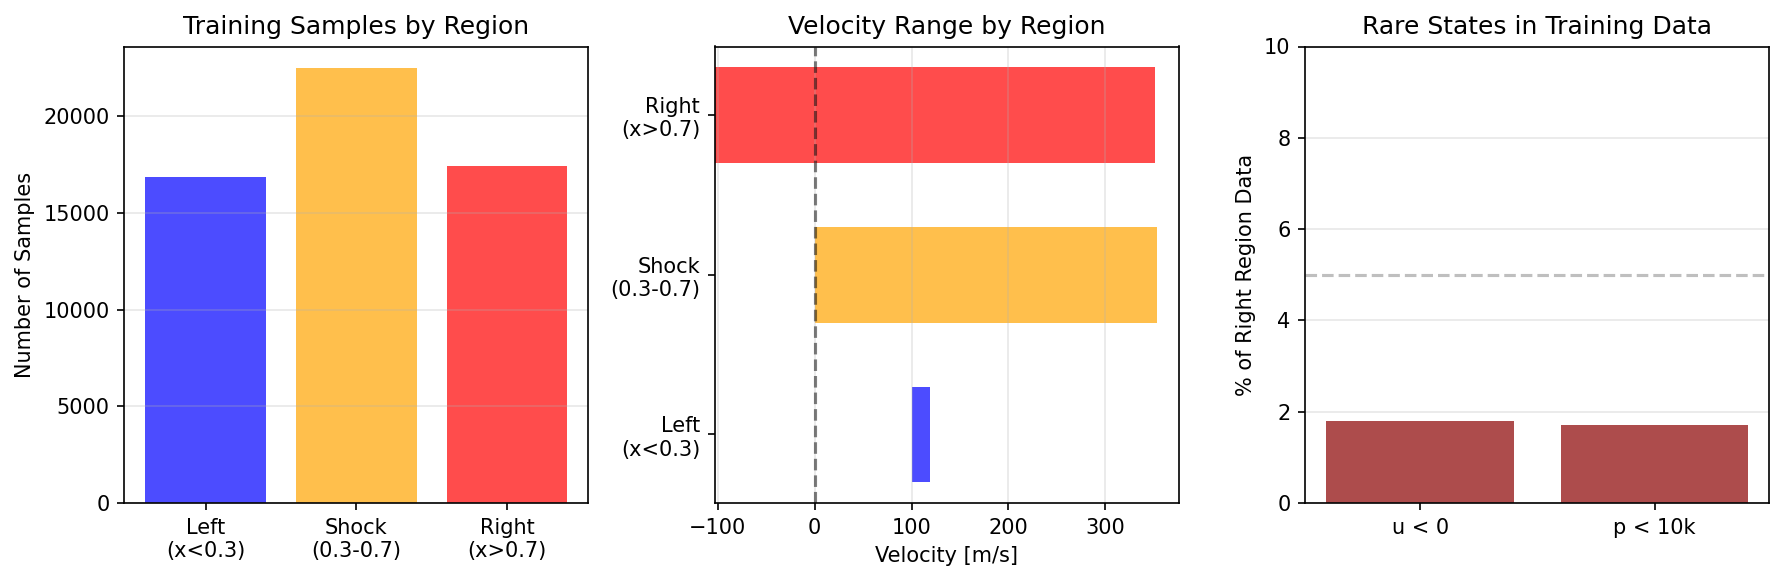
\includegraphics[width=\textwidth]{training_data_distribution.png}
    \caption{Training data distribution showing rare extreme states.}
    \label{fig:data_dist}
\end{figure}

\begin{table}[H]
\centering
\begin{tabular}{lcc}
\toprule
Condition & Samples & \% of Right Region \\
\midrule
$\rho < 0.15$ & 12,059 & 69\% (adequate) \\
$u < 0$ (negative velocity) & 315 & \textbf{1.8\%} (rare) \\
$p < 10,000$ Pa & 296 & \textbf{1.7\%} (rare) \\
\bottomrule
\end{tabular}
\caption{Representation of extreme states in training data.}
\label{tab:imbalance}
\end{table}

\section{Experiments}

\subsection{Conservation Constraints}

We tested multiple approaches to enforce physical conservation laws. All degraded performance:

\begin{table}[H]
\centering
\begin{tabular}{lcc}
\toprule
Approach & Validation Loss & Result \\
\midrule
Baseline (no constraints) & $5.5 \times 10^{-5}$ & Stable \\
Hard antisymmetric ($F_{ij} = -F_{ji}$) & $3.84 \times 10^{-3}$ & \textbf{Exploded} \\
Soft conservation ($\lambda = 0.1$) & $9.5 \times 10^{-5}$ & Errors doubled \\
Soft conservation ($\lambda = 0.01$) & $8.5 \times 10^{-5}$ & Unstable \\
Global conservation ($\lambda = 0.01$) & $5.2 \times 10^{-5}$ & Unstable \\
Global conservation ($\lambda = 0.001$) & $8.6 \times 10^{-5}$ & Unstable \\
\bottomrule
\end{tabular}
\caption{Conservation constraint experiments. All approaches failed.}
\label{tab:conservation}
\end{table}

\textbf{Conclusion}: The Roe flux is not antisymmetric by design. Conservation emerges naturally from the finite volume update structure. Adding constraints degrades performance.

\subsection{Residual Connections and LayerNorm}

Adding residual blocks with LayerNorm and GELU activation provided marginal improvement:

\begin{table}[H]
\centering
\begin{tabular}{lcc}
\toprule
Metric & Baseline & Residual + LayerNorm \\
\midrule
Validation Loss & $5.5 \times 10^{-5}$ & $8.1 \times 10^{-5}$ \\
Training Loss & $5.7 \times 10^{-5}$ & $2.8 \times 10^{-5}$ \\
Density RMS & $5 \times 10^{-2}$ & $5.16 \times 10^{-2}$ \\
Velocity RMS & 48 & 53.8 \\
Pressure RMS & 5,500 & 4,350 \\
\bottomrule
\end{tabular}
\caption{Effect of residual connections and LayerNorm.}
\label{tab:residual}
\end{table}

\subsection{Finer Grid (400 Nodes)}

Attempting 4$\times$ finer resolution failed due to the Gibbs phenomenon:
\begin{itemize}
    \item More edges around the shock = more extreme flux gradients
    \item Fewer total samples due to CFL-constrained timestep
    \item Simulation became unstable
\end{itemize}

\section{Conclusions}

\begin{enumerate}
    \item \textbf{Standard MSE loss works best} -- no conservation constraints needed
    \item \textbf{Architecture changes provide marginal improvement} -- the bottleneck is data, not model capacity
    \item \textbf{Finer grids don't help} -- Gibbs phenomenon makes shock regions harder to learn
    \item \textbf{Primary error source is training data imbalance} -- extreme boundary states (negative velocity, low pressure) are underrepresented
\end{enumerate}

\section{Recommendations}

For future improvement:
\begin{itemize}
    \item Generate more diverse training data with different initial conditions
    \item Add shock-aware features (gradient magnitude)
    \item Use importance sampling to oversample rare states
    \item Consider hybrid approaches: GNN for smooth regions, classical Roe flux near discontinuities
\end{itemize}

\end{document}
